\usetikzlibrary{arrows.meta,matrix,positioning}

% FIXME: explain we are using VIRTUAL TAGS
% FIXME: explain aliasing problem with one set
\begin{frame}{virtual caches: aliasing problem}
    \begin{itemize}
        \item two virtual addresses can map to same physical
        \item problem for caches with virtual indexes+tags
        \vspace{.5cm}
        \item say VA 0x1000 and 0x2000 map to same physical
        \item what happens if application writes to 0x1000
        \item \ldots then reads from 0x2000?
    \end{itemize}
\end{frame}

\begin{frame}{virtual cache aliasing solutions}
    \begin{itemize}
    \item software solution: OS promises not to have aliasing
    \item hardware solution: hardware detects aliasing
        \begin{itemize}
        \item requires extra bookkeeping
        \end{itemize}
    \end{itemize}
\end{frame}

\begin{frame}[fragile,label=hwAlias]{hardware alias detection (1)}
    \begin{itemize}
    \item key idea: store physical address \textit{and virtual-address-based tag}
    \item store value? check for other copies of same physical addr
    \item if found: evict other copies
    \end{itemize}
\begin{tikzpicture}
\tikzset{
    v/.style={visible on=<#1->,alt=<#1>{red}},
    h/.style={alt=<#1>{red}},
    tagColor/.style={color=green!60!black},
    physColor/.style={color=red!60!black},
    dataColor/.style={color=blue!60!black},
    offsetColor/.style={color=yellow!30!black},
}
\matrix[tight matrix,
        nodes={font=\small\tt,text depth=.1ex,text height=1ex,minimum height=.5cm},
        row 1/.append style={nodes={font=\small\bfseries,minimum height=.5cm}},
        column 1/.append style={nodes={draw=none,text width=1.2cm}},
        column 2/.append style={nodes={align=center,text width=.5cm}},
        column 3/.append style={nodes={align=center,tagColor,text width=2cm}},
        column 4/.append style={nodes={align=center,physColor,text width=2cm}},
        column 5/.append style={nodes={text width=1cm,align=center,dataColor}},
        column 6/.append style={nodes={draw=none,text width=.1cm}},
        column 7/.append style={nodes={align=center,text width=.5cm}},
        column 8/.append style={nodes={align=center,tagColor,text width=2cm}},
        column 9/.append style={nodes={align=center,physColor,text width=2cm}},
        column 10/.append style={nodes={text width=1cm,align=center,dataColor}},
       ] (cache)  {
           index \& V \& tag \& phys addr \& value \& ~ \& V \& tag \& phys addr \& value \\
0\&
    % i 0, 0:
    1 \& 
    0x03312 \&
    0x1F4300 \&
    \ldots \&  ~ \&
    % i 0, 1:
    1 \&
    0x03311 \&
    0x1F3400 \&
    \ldots \\
1\& 
    % i 1, 0:
    1 \&
    0x7FF33 \&
    0x183220 \&
    \ldots \& ~ \& 
    % i 1, 1:
    1 \&
    0x03310 \&
    0x0F3A20 \&
    \ldots \\
2\& 
    % i 1, 0:
    1 \&
    0x7FF33 \&
    0x183240 \&
    \ldots \& ~ \& 
    % i 1, 1:
    1 \&
    0x03320 \&
    0x030040 \&
    \ldots \\
\ldots \\
};
\end{tikzpicture}
\end{frame}

\begin{frame}{checking all the physical addresses? (1)}
    \begin{itemize}
    \item scanning entire cache for same physical address?
    \item do we really need to scan everything?
    \vspace{.5cm}
\item<2-> exercise(1): if we have 4096 ($2^{12}$) byte pages, give an example of a virtual address that could
          map to the same physical as \texttt{0x12010}?
    \iftoggle{heldback}{}{
    \item<3-> must have same page offset, so 0x0010, 0x1010, 0x2010, 0x3010, etc.
    }
    \end{itemize}
\end{frame}
\begin{frame}{checking all the physical addresses? (2)}
    \begin{itemize}
    \item scanning entire cache for same physical address?
    \item do we really need to scan everything?
    \vspace{.5cm}
    \item with 4K pages ($2^{12}$ byte):
    \item exercise(2): if we have a direct-mapped 4K \textbf{virtual} cache with 16 byte blocks,
          in which sets can be these aliasing addresses be stored?
    \end{itemize}
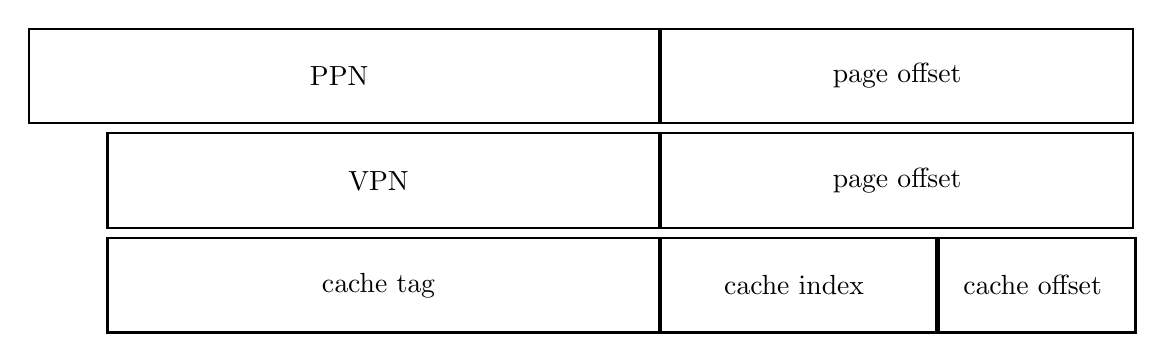
\begin{tikzpicture}
\tikzset{
    ht/.style={draw,thick,minimum height=1.2cm,align=center,inner sep=0mm},
}
\node[ht,minimum width=8cm,anchor=north west] (ppn) { PPN };
\node[ht,minimum width=7cm,anchor=north east] (vpn) at ([yshift=-.1cm]ppn.south east){ VPN };
\node[ht,right=0cm of ppn,minimum width=6cm] {page offset};
\node[ht,right=0cm of vpn,minimum width=6cm] {page offset};
\node[ht,minimum width=7cm,anchor=north west] (cacheTag) at ([yshift=-.1cm,xshift=0cm]vpn.south west){ cache tag };
\node[ht,minimum width=3.5cm,right=0cm of cacheTag] (cacheIndex) { cache index };
\node[ht,minimum width=2.5cm,right=0cm of cacheIndex] (cacheOff) { cache offset };
\end{tikzpicture}
\end{frame}

\begin{frame}{checking all the physical addresses? (3)}
    \begin{itemize}
    \item scanning entire cache for same physical address?
    \item do we really need to scan everything?
    \vspace{.5cm}
    \item exercise(3): if we have a direct-mapped \textbf{8K} \textbf{virtual} cache with 16-byte blocks,
         in which sets can these aliasing addresses be stored?
    \end{itemize}
\begin{tikzpicture}
\tikzset{
    ht/.style={draw,thick,minimum height=1.2cm,align=center,inner sep=0mm},
}

\node[ht,minimum width=8cm,anchor=north west] (ppn) { PPN };
\node[ht,minimum width=7cm,anchor=north east] (vpn) at ([yshift=-.1cm]ppn.south east){ VPN };
\node[ht,right=0cm of ppn,minimum width=5cm] {page offset};
\node[ht,right=0cm of vpn,minimum width=5cm] {page offset};
\node[ht,minimum width=6cm,anchor=north west] (cacheTag) at ([yshift=-.1cm,xshift=0cm]vpn.south west){ cache tag };
\node[ht,minimum width=3.5cm,right=0cm of cacheTag] (cacheIndex) { cache index };
\node[ht,minimum width=2.5cm,right=0cm of cacheIndex] (cacheOff) { cache offset };
\begin{visibleenv}<2>
    \draw[red,dotted,line width=4pt] (vpn.north east |- ppn.north) rectangle (cacheIndex.south west);
\end{visibleenv}
\end{tikzpicture}
\end{frame}

\begin{frame}{virtual caches: detecting aliasing}
    \begin{itemize}
    \item suppose two virtual addresses with same physical address
    \item addrs differ only VPN bits
    \item finding which indexes to check: worry about overlap:
    \end{itemize}
\begin{tikzpicture}
\tikzset{
    ht/.style={draw,thick,minimum height=1.2cm,align=center,inner sep=0mm},
}

\node[ht,minimum width=8cm,anchor=north west] (ppn) { PPN };
\node[ht,minimum width=7cm,anchor=north east] (vpn) at ([yshift=-.1cm]ppn.south east){ VPN };
\node[ht,right=0cm of ppn,minimum width=5cm] {page offset};
\node[ht,right=0cm of vpn,minimum width=5cm] {page offset};
\node[ht,minimum width=6cm,anchor=north west] (cacheTag) at ([yshift=-.1cm,xshift=0cm]vpn.south west){ cache tag };
\node[ht,minimum width=3.5cm,right=0cm of cacheTag] (cacheIndex) { cache index };
\node[ht,minimum width=2.5cm,right=0cm of cacheIndex] (cacheOff) { cache offset };
\begin{visibleenv}<2>
    \draw[red,dotted,line width=4pt] (vpn.north east |- ppn.north) rectangle (cacheIndex.south west);
\end{visibleenv}
\end{tikzpicture}
\end{frame}

\begin{frame}{virtual caches: aliasing detection outline}
    \begin{itemize}
    \item hardware alias detection mechanism
    \vspace{.5cm}
    \item store physical address of each block in the cache
        \begin{itemize}
            \item \ldots in addition to virtual tag
        \end{itemize}
    \item when adding value to cache, try \myemph{all other indexes for same page offset}
    \item if any match physical address: evict that copy
    \item result: only store one virtual address per physical address at a time
    \item actual strategy used by AMD Opteron's instruction cache
        \begin{itemize}
        \item 2 cache index bits overlapping VPN
        \item 4 cache sets to check on cache replacement
        \item (also on conflicting writes to data cache?)
        \end{itemize}
    \end{itemize}
\end{frame}
